\documentclass[11pt]{article}
\usepackage[utf8]{inputenc}
\usepackage{hyperref}
\usepackage{mathtools, amssymb}
\usepackage{tikz}

\title{The pendulum problem and elliptic integrals}
\author{Max Levine}
\date{\today}

\setlength{\parindent}{0pt}

\begin{document}
\maketitle
\tableofcontents

\section{Introduction}
This paper is a collection of notes based on an interesting video I watched with my friend, and a series of seminars given by my cal 3 teacher in college. I will reveal the connections between pendulums in physics, elliptic integrals, functional equations, the arithmetic-geometric mean, and more.

\vspace{5mm} I will present these topics in the way that I discovered them, starting with the example of finding the period of a pendulum, then moving on to functional equations and elliptic integrals. 

\section{The pendulum problem}
\subsection{The problem}
This first part is based on the \underline{\href{https://www.youtube.com/watch?v=h19xcTPzlEc}{video}} my friend and I found titled: The complete elliptic integral of the first kind.
The problem: find the period of a pendulum.

\vspace{10mm}\begin{minipage}{6cm}
We've all learned in mechanics class that the period of a pendulum can be found using the equation
$$T=2\pi\sqrt{\dfrac{L}{g}}$$
\end{minipage} \quad
\fbox{
\begin{minipage}{6cm}
\begin{center}
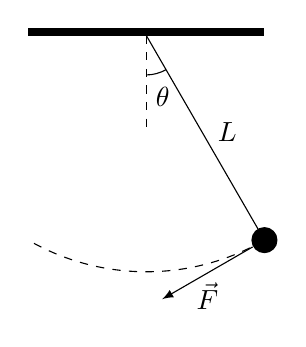
\begin{tikzpicture}
% Support
\fill (-1.5,0) rectangle(1.5,0.1);

\draw[dashed] (-60:3) arc(-60:-120:3);

\draw (0,0) -- (-60:3) node[fill,circle](m){};
\draw (0,0)[dashed] -- (-90:1.2);
\node at (-50:1.6) {$L$};
\node at (-75:0.8) {$\theta$};
\draw (-60:0.5) arc(-60:-90:0.5);

% Force
\draw[-latex] (m) -- node[below]{$\vec{F}$}++(210:1.5);
\end{tikzpicture}

A simple mechanical pendulum
\end{center}
\end{minipage} }

\vspace{5mm}However this formula is only accurate for small values of $\theta$, so it's only natural to wonder at what the real period formula looks like.

\subsection{Setting up the integral}
The guy starts off the video by showing the titular \textbf{complete elliptic integral of the first kind}, which looks like
$$K(n)=\int_0^{\frac{\pi}{2}}\frac{d\theta}{\sqrt{1-n^2\sin^2\theta}}$$

He claims that this integral appears as a solution for certain physics problems such as a pendulum problem. Sounds believable enough. He also mentions that he will be looking at some interesting values of this function.

\vspace{5mm} The setup is as follows:

\begin{center}
\begin{tikzpicture}
\draw (0,0) -- (5,0) node[right]{$x$};
\draw (0,0) -- (0,-4) node[below]{$y$};

\draw (0,0) -- (-50:3) node[fill,circle](m){};
\draw[dashed] (-50:3) arc(-50:-90:3);
\draw (0,0)[dashed] -- (-90:1.2);
\node at (-40:1.5) {$l$};
\node at (-70:0.8) {$\varphi_0$};
\draw (-50:0.5) arc(-50:-90:0.5);

%\draw[-latex] (m) -- node[below]{$\vec{F}$}++(220:1.5);
\end{tikzpicture}
\end{center}

A pendulum of mass $m$, attached to a string of length $l$, oscillating with an amplitude of $\varphi_0$

\vspace{5mm} We look at the energy of the pendulum at an angle $\varphi$. The $x$-axis is set as the level of $0$ gravitational potential energy. 

\vspace{5mm}The kinetic energy $K=\frac{1}{2}mv^2$ and the potential energy $U=-mgl\cos\varphi$. If energy is conserved then the total energy of the pendulum at any point is
$$E=-mgl\cos\varphi_0=\frac{1}{2}mv^2-mgl\cos\varphi$$
Where the velocity $v$ is defined as the derivative of the arc length 
$$v=\frac{ds}{dt}=\frac{ld\varphi}{dt}$$
So we have the differential equation
$$E=-mgl\cos\varphi_0=\frac{1}{2}ml^2\dot\varphi^2-mgl\cos\varphi$$
And we can rearange to get
\begin{gather*}
\frac{1}{2}ml^2\dot\varphi^2=mgl(\cos\varphi-\cos\varphi_0) \\
\frac{1}{2}l\dot\varphi^2=g(\cos\varphi-\cos\varphi_0) \\
\dot\varphi^2=\frac{2g}{l}(\cos\varphi-\cos\varphi_0) \\
\frac{d\varphi}{dt}=\sqrt{\frac{2g}{l}(\cos\varphi-\cos\varphi_0)}
\end{gather*}

So far pretty simple, only some basic knowledge in mechanics and calculus required.

\vspace{5mm} Since we are trying to find the period, we isolate $dt$ and integrate.

$$\int dt=\sqrt{\frac{l}{2g}}\int\frac{d\varphi}{\sqrt{(\cos\varphi-cos\varphi_0)}}$$

The pendulum takes a quarter period to move from $0$ to $\varphi_0$ so we get
$$\frac{T}{4}=\sqrt{\frac{l}{2g}}\int_0^{\varphi_0}\frac{d\varphi}{\sqrt{(\cos\varphi-cos\varphi_0)}}$$

And so the true formula for the period of the pendulum is 

$$T=2\sqrt{2}\sqrt{\frac{l}{g}}\int_0^{\varphi_0}\frac{d\varphi}{\sqrt{(\cos\varphi-cos\varphi_0)}}$$

\subsection{Start substituting}

But wait, I thought the solution was going to look something like our elliptic integral
$\int\frac{d\theta}{\sqrt{1-n^2\sin^2\theta}}$?

\vspace{5mm} We are going to have to make a few substitutions.

First, the identity $\cos(2\varphi)=1-2\sin^2\varphi \longrightarrow \cos\varphi=1-2\sin^2\frac{\varphi}{2}$

$$T=2\sqrt{2}\sqrt{\frac{l}{g}}\int_0^{\varphi_0}\frac{d\varphi}{\sqrt{(1-2\sin^2\frac{\varphi}{2}-cos\varphi_0)}}$$

\section{Functional Equations}
In order to understand the solution above, we must talk about functional equations. Functional equations are similar to differential equations in that their solutions are functions themselves. Consider the functional equation

$$f(xy)=f(x)+f(y)$$

You might know a function that solves this equation, but for the moment, pretend we don't know what that function is, what can we say about this function?

\vspace{5mm} If we take $x=0,y=0$ then we see that $f(0)=f(0)+f(0)\Rightarrow f(0)=0$



\begin{thebibliography}{9}

\bibitem{thing}
\emph{Title}, Website Title
\url{real}

\end{thebibliography}

\end{document}
